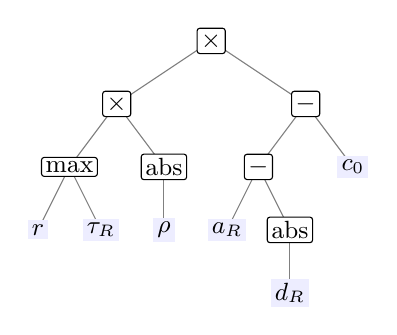
\begin{tikzpicture}[x=8mm,y=8mm,every node/.style={font=\small,inner sep=1.5pt}]
\draw[gray] (0.5,-2) -- (0,-3);
\draw[gray] (0.5,-2) -- (1,-3);
\draw[gray] (2.0,-2) -- (2,-3);
\draw[gray] (1.25,-1) -- (0.5,-2);
\draw[gray] (1.25,-1) -- (2.0,-2);
\draw[gray] (4.0,-3) -- (4,-4);
\draw[gray] (3.5,-2) -- (3,-3);
\draw[gray] (3.5,-2) -- (4.0,-3);
\draw[gray] (4.25,-1) -- (3.5,-2);
\draw[gray] (4.25,-1) -- (5,-2);
\draw[gray] (2.75,0) -- (1.25,-1);
\draw[gray] (2.75,0) -- (4.25,-1);
\node[fill=blue!7] at (0,-3) {$r$};
\node[fill=blue!7] at (1,-3) {$\tau_R$};
\node[draw,rounded corners=1pt,fill=white] at (0.5,-2) {$\max$};
\node[fill=blue!7] at (2,-3) {$\rho$};
\node[draw,rounded corners=1pt,fill=white] at (2.0,-2) {$\mathrm{abs}$};
\node[draw,rounded corners=1pt,fill=white] at (1.25,-1) {$\times$};
\node[fill=blue!7] at (3,-3) {$a_R$};
\node[fill=blue!7] at (4,-4) {$d_R$};
\node[draw,rounded corners=1pt,fill=white] at (4.0,-3) {$\mathrm{abs}$};
\node[draw,rounded corners=1pt,fill=white] at (3.5,-2) {$-$};
\node[fill=blue!7] at (5,-2) {$c_{0}$};
\node[draw,rounded corners=1pt,fill=white] at (4.25,-1) {$-$};
\node[draw,rounded corners=1pt,fill=white] at (2.75,0) {$\times$};
\end{tikzpicture}
